\chapter{KAJIAN PUSTAKA}

\section{Penelitian Terdahulu}
\begin{longtable}{|P{0.25\linewidth}|P{0.25\linewidth}|P{0.25\linewidth}|P{0.25\linewidth}|}
\caption{Tinjauan Penelitian Terdahulu} \label{tab:penelitian_terdahulu_simple} \\
\hline
\textbf{Studi} & \textbf{Fokus} & \textbf{Metode utama} & \textbf{Hasil/Output} \\ \hline
\endfirsthead

\multicolumn{4}{l}{\textit{Tabel \ref{tab:penelitian_terdahulu_simple} (lanjutan).}}\\
\hline
\textbf{Studi} & \textbf{Fokus} & \textbf{Metode utama} & \textbf{Hasil/Output} \\ \hline
\endhead

\hline
\multicolumn{4}{r}{\textit{Bersambung ke halaman berikutnya}} \\
\endfoot

\hline
\endlastfoot

% Entri 1
\textbf{Judul:} \textit{Knowledge Graph Generation and Application for Unstructured Data Using Data Processing Pipeline} \newline
\textbf{Penulis:} Sukumar, dkk. (2024)
& 
Membangun dan mengevaluasi pipeline \textit{end-to-end} untuk konstruksi Knowledge Graph (KG) dari teks tidak terstruktur. Fokusnya adalah membandingkan dua teknik Ekstraksi Relasi (RE).
& 
Menggunakan pipeline NLP (Coreference Resolution, Named Entity Linking, RE) dan database graf Neo4j. \newline
\textbf{Perbandingan:} Model OpenNRE (\textit{few-shot}) vs REBEL (\textit{Seq2Seq}).
& 
REBEL (akurasi 87\%) mengungguli OpenNRE (61.4\%). REBEL juga lebih cepat (1 jam vs 3 jam).
\\ \hline

% Entri 2
\textbf{Judul:} \textit{Open-Source Agentic Hybrid RAG Framework for Scientific Literature Review} \newline
\textbf{Penulis:} Nagori, dkk. (2025)
& 
Mengembangkan kerangka kerja RAG hibrida yang bersifat \textit{agentic} (otonom) untuk tinjauan literatur ilmiah. Agen AI secara dinamis memilih mode \textit{retrieval} (GraphRAG vs VectorRAG).
& 
Menggunakan agen AI (Llama-3.3-70B) untuk memilih antara: \newline
1) \textbf{GraphRAG} Kueri Cypher ke Neo4j \newline
2) \textbf{VectorRAG} Pencarian hibrida di FAISS VS. \newline
Dilakukan \textit{Instruction Tuning} dengan DPO.
& 
Agen (dengan DPO) secara signifikan mengungguli RAG non-agentic. \newline
\textbf{Gain:} \newline
+0.63 \textit{VS Context Recall} \newline
+0.56 \textit{overall Context Precision}
\\ \hline
\end{longtable}
		
\section{Kajian Teori}

\subsection{Scholarly Search}
Pertumbuhan pesat dalam volume publikasi ilmiah menciptakan tantangan informasi yang signifikan bagi para peneliti. Untuk mengatasi masalah ini, berbagai sistem pencarian akademik telah dikembangkan termasuk \textit{Google Scholar, Semantic Scholar, AMiner, Xueshu Baidu, Microsoft Academic Search, CiteSeerX}, dan platform-platform lainnya \cite{10.1007/s11192-020-03690-4}. Di antara semua platform ini, \textit{Google Scholar} mendominasi dengan cakupan literatur paling luas. Namun, cakupan yang luas saja tidak selalu menjamin efektivitas, khususnya ketika peneliti mencari dokumen yang benar-benar relevan dengan kebutuhan mereka. Dalam konteks ini, mekanisme perangkingan dokumen menjadi aspek krusial yang sering kali menentukan kualitas hasil pencarian.

Masalah utama yang dihadapi sistem pencarian akademik konvensional adalah ketergantungan pada jumlah sitasi untuk merangking makalah dalam daftar kandidat yang relevan. Ketika mekanisme perangkingan tidak efektif, terjadi kecenderung beralih ke platform pencarian lain seperti \textit{PubMed, Microsoft Academic Search, atau Semantic Scholar} \cite{https://doi.org/10.1609/aimag.v36i3.2601, 10.1145/1401890.1402008, 10.1145/2740908.2742839, Lu2011, 10.1145/3038912.3052558}. Platform-platform alternatif ini mengimplementasikan berbagai teknik analitik untuk meningkatkan kualitas hasil pencarian, termasuk disambiguasi nama penulis \cite{10.1145/1401890.1402008}, mengukur tingkat signifikansi publikasi \cite{Shen2016ModelingTA}, dan merangkum publikasi berdasarkan entitas-entitas kunci \cite{ren-etal-2017-life}.

Pertanyaan penelitian yang paling mendesak dalam pencarian akademik adalah bagaimana mendefinisikan dan mengukur kesamaan serta relevansi antara dua artikel dengan mempertimbangkan kueri pencarian tertentu. Beberapa pendekatan terdahulu mencoba mengatasi ini dengan memanfaatkan informasi tekstual dan struktural secara bersama-sama. Misalnya, Mai et al. mengusulkan penggunaan embeddings tekstual dan struktural untuk menemukan makalah yang relevan dengan kueri yang diberikan. Namun pendekatan tersebut memerlukan data pelatihan dan penyetelan parameter dalam pengambilan literatur secara terawasi (supervised learning), berbeda dengan pendekatan yang tidak memerlukan pelatihan khusus (unsupervised approach) seperti yang disarankan dalam penelitian ini.

\subsection{Knowledge Graph}

\textit{Knowledge Graph} (KG) atau Graf Pengetahuan merupakan pendekatan terstruktur dalam merepresentasikan pengetahuan yang mengaitkan beragam entitas beserta relasinya dalam sebuah bentuk yang terstruktur. Secara matematis, KG dimodelkan sebagai graf berarah $G = (E, R, T)$, di mana $E$ mewakili sebuah entitas (misalnya individu, konsep, atau peristiwa), $R$ mewakili sebuah relasi seperti "mengajar", "bagian\_dari", atau "berafiliasi\_dengan", dan $T \subseteq E \times R \times E$ merepresentasikan sebuah triplet \cite{Hogan_2021}. Setiap triplet $(h, r, t) \in T$ merangkum satu pengetahuan contohnya entitas kepala (\textit{head}) $h$ terhubung secara relasional dengan entitas ekor (\textit{tail}) $t$ melalui relasi $r$. Sebagai ilustrasi, triplet (Jakarta, IBUKOTA, Indonesia) atau (Prabowo, Presiden, Indonesia) mengabstraksikan relasi yang dalam domain geopolitik. Struktur berbasis graf ini memungkinkan adanya penalaran, penelusuran, dan pengintegrasian sumber data heterogen secara efektif, yang membuat KG menjadi tak tergantikan dalam sistem pemahaman semantik dan dalam pengambil sebuah keputusan.
		
Pembangunan KG melibatkan beberapa tahapan utama. Tahap awal adalah akuisisi pengetahuan melalui ekstraksi dari sumber teks tidak terstruktur menggunakan teknik \textit{Natural Language Processing} (NLP) seperti \textit{Named Entity Recognition} untuk mengidentifikasi berbagai entitas dan \textit{Relation Extraction} untuk menemukan relasi di antara entitas dan mengintegrasikan dengan data terstruktur dari basis-basis pengetahuan yang sudah ada (misal Wikidata \cite{wikidata}) yang bertujuan memperluas cakupan Knowledge. KG yang telah terbentuk dapat diperkaya melalui pendekatan seperti (\textit{link prediction}) atau penalaran berbasis aturan untuk menginferensi fakta baru. Misalnya, KnowEdu yang berfokus di bidang pendidikan menggunakan teknik \textit{neural sequence labeling} dan aturan asosiasi probabilistik untuk mengekstraksi konsep-konsep pedagogis serta hubungan prasyaratnya dari data kurikulum \cite{knowedu}.Saat ini, dengan kemajuan pesat Model Bahasa Besar dalam pemahaman semantik dan ekstraksi entitas, berbagai penelitian mulai memanfaatkan LLM untuk mengotomatisasi serta meningkatkan akurasi proses pembangunan KG \cite{edge2025localglobalgraphrag}.
		
Knowledge Graph telah diterapkan secara luas di berbagai bidang karena kemampuannya yang unggul dalam merepresentasikan hubungan kompleks serta mengintegrasikan berbagai sumber data heterogen:  
\begin{daftar}
	\item Mesin Pencarian dan Pengambilan Informasi: Platform komersial seperti KG Google memanfaatkan hubungan antar entitas untuk memperjelas kueri dan menyediakan informasi kontekstual, yang secara signifikan meningkatkan akurasi pencarian dalam pengujian standar.  
	\item Recommendation Systems: KGs mendukung mesin rekomendasi dengan mengidentifikasi keterkaitan antara preferensi pengguna dan konten, sehingga menghasilkan saran yang lebih relevan.
	\item Healthcare: Knowledge Graphs (KGs) mengintegrasikan sejumlah besar data biomedis, yang membantu dalam penemuan obat, penelitian penyakit, dan pengobatan yang dipersonalisasidengan mengungkap relasi tersembunyi antara entitas biologis.
\end{daftar}

Berbagai penerapan terbaru telah mengintegrasikan Knowledge Graph (KG) dengan Large Language Models (LLM) untuk meningkatkan kemampuan penalaran serta kemampuan LLM dalam menghasilkan jawaban. Contohnya, arsitektur DRAGON \cite{yasunaga2022deepbidirectionallanguageknowledgegraph} berhasil mencapai performa terbaik pada benchmark pertanyaan kompleks seperti CSQA dan OBQA, dengan melatih LLM menggunakan data dari KG sehingga memungkinkan LLM memberikan jawaban yang terstruktur terhadap pertanyaan yang kompleks \cite{saha2018complexsequentialquestionanswering, mihaylov2018suitarmorconductelectricity}. Ke depannya, pengembangan KG diperkirakan akan berfokus pada konstruksi berbasis input multimodal dan eksplorasi embedding graf untuk mendukung pengambilan keputusan secara real-time.

\subsection{Graf Basis Data dalam Riset Akademik}

Graf basis data telah menjadi instrumen penting untuk memodelkan dan mengeksplorasi relasi dalam data akademik. Dalam representasi berbasis graf, node dapat merepresentasikan berbagai entitas seperti publikasi, peneliti, institusi, atau konsep ilmiah utama, sementara edge menangkap relasi seperti ``Publikasi A mengutip Publikasi B'', ``Peneliti X berkolaborasi dengan Peneliti Y'', atau ``Topik Z terkait dengan Metode Y''. Format ini secara alamiah mencerminkan struktur ekosistem pengetahuan ilmiah. Sebagai contoh, jaringan sitasi membentuk graf berarah (\textit{directed graph}), dan jejaring kolaborasi peneliti membentuk graf co-authorship. Knowledge graph (KG) juga dapat mengenkode koneksi tingkat lebih tinggi, misalnya sebuah ``graf topik'' dapat menghubungkan publikasi dengan area riset atau metodologi yang digunakan.

Graf basis data seperti Neo4j sangat sesuai untuk menyimpan dan melakukan query terhadap jaringan semacam ini karena kemampuannya dalam melakukan penelusuran relasi (\textit{relationship traversal}) secara efisien. Penggunaan model berbasis graf dalam riset akademik menawarkan kapabilitas yang powerful untuk \textit{literature mining} dan \textit{knowledge discovery}. Iancarelli \textit{et al.} membangun graf sitasi dari literatur riset agresi manusia untuk memetakan struktur tematiknya. Analisis mereka menemukan klaster-klaster yang berbeda (misalnya, media dan video game, pengaruh hormon) dan mengidentifikasi paper-paper ``jembatan'' (\textit{bridging papers}) yang menghubungkan berbagai komunitas riset \cite{pub.1147279270}. Proyek seperti Open Research Knowledge Graph (ORKG) merepresentasikan kontribusi inti dari paper dalam bentuk terstruktur, membuat pengetahuan ilmiah dapat diakses dan diproses secara otomatis oleh mesin \cite{Jaradeh_2019}.

Dengan mengkurasi paper-paper ke dalam KG yang berisi konsep dan relasi, peneliti dapat melakukan query seperti ``publikasi mana yang menggunakan metode X dan mencapai hasil Y?'' sebuah tugas yang sulit dilakukan dengan teks tidak terstruktur. Dalam konteks institusi seperti UNESA, graf basis data memungkinkan eksplorasi relasi kompleks yang tidak dapat ditangkap oleh sistem pencarian konvensional. Sebagai contoh, pertanyaan ``siapa peneliti di Infokom yang aktif dalam topik Machine Learning dan pernah berkolaborasi dengan institusi luar negeri dalam 5 tahun terakhir?'' membutuhkan penelusuran \textit{multi-hop} pada graf yang menghubungkan node peneliti, topik, publikasi, dan afiliasi. Knowledge graph berbasis Neo4j dapat menjawab query semacam ini dengan efisien melalui \textit{Cypher queries}, sekaligus menyediakan visualisasi jejaring kolaborasi dan pola tren riset yang tidak mudah terlihat dari data tabular atau sistem pencarian berbasis kata kunci.

\begin{figure}[!t]
    \centering
    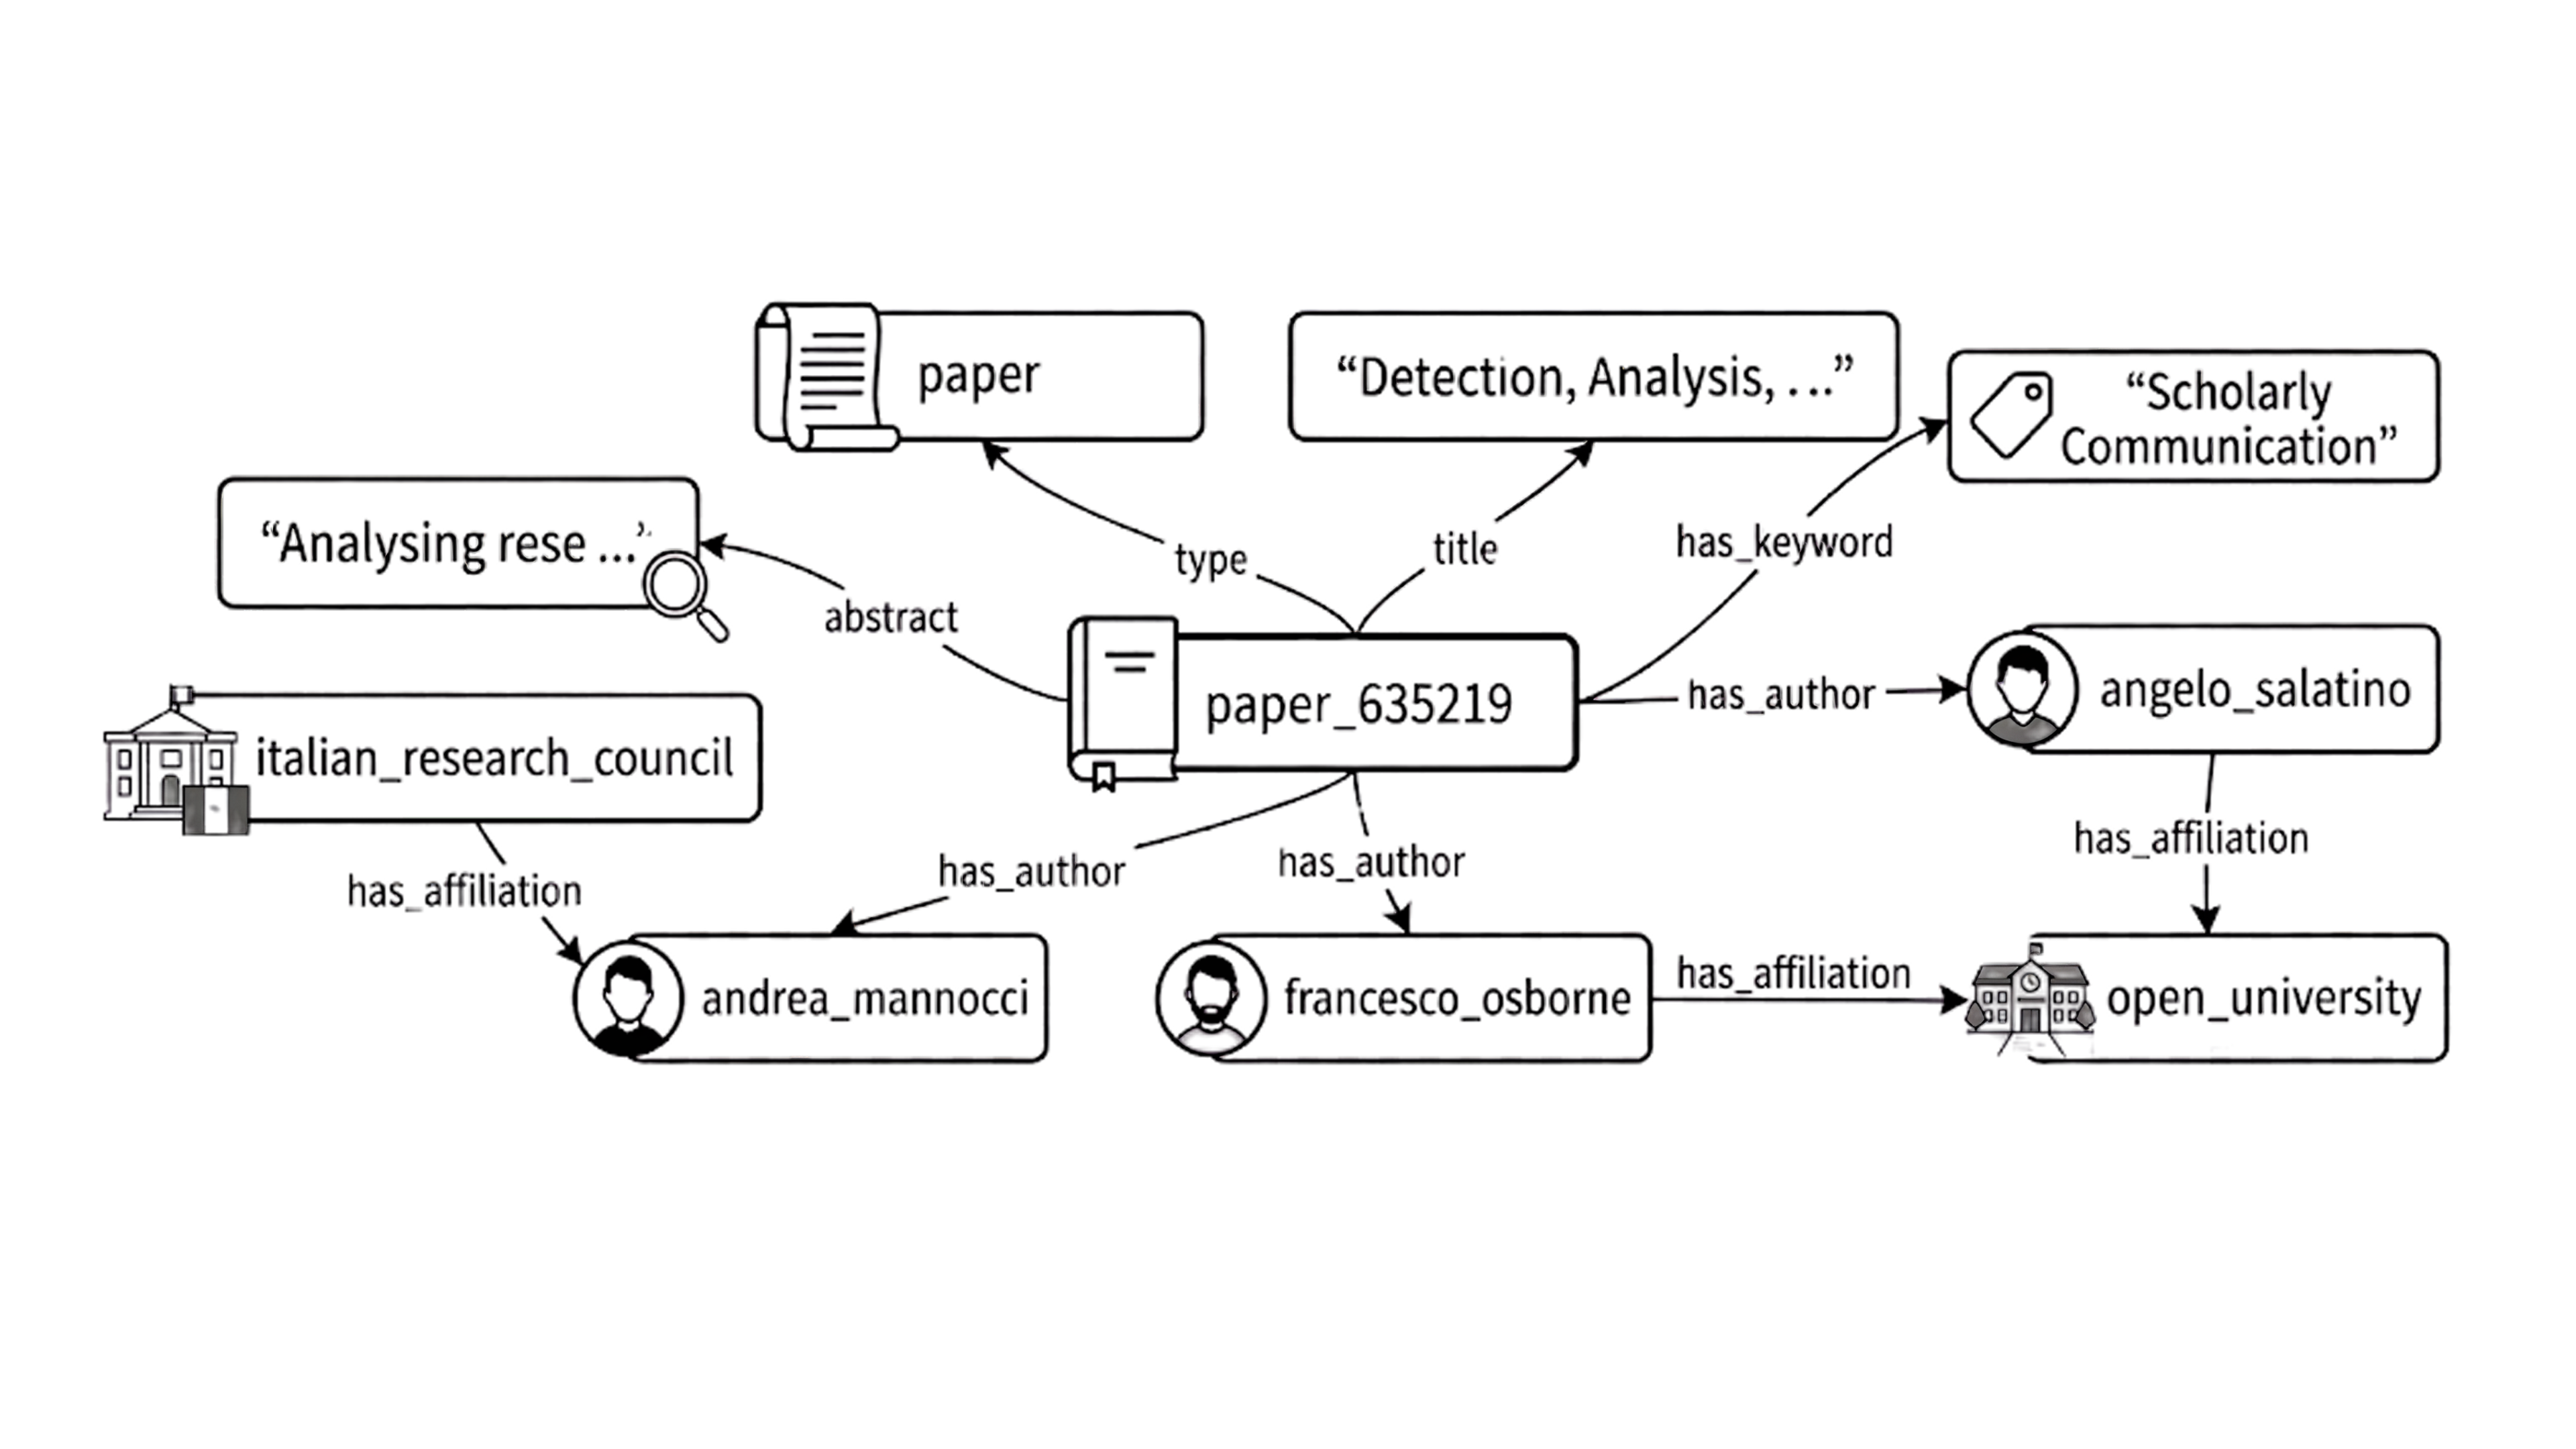
\includegraphics[width=0.9\textwidth]{Gambar/Untitled design.png}
    \caption{Knowledge Graph untuk domain penelitian akademik}
    \label{fig:kg-academic}
\end{figure}

\subsection{NLP}



\subsection{LLM}
Large Language Models (LLM) merupakan model pembelajaran mendalam yang dilatih pada volume besar data teks sehingga mampu memahami dan menghasilkan teks yang mirip dengan tulisan manusia. Model ini dibangun dengan arsitektur Transformer yang memanfaatkan mekanisme self-attention untuk memproses urutan data dan menangkap hubungan jangka panjang antar elemen teks \cite{vaswani2023attentionneed}. Berkat mekanisme tersebut, LLM modern menunjukkan performa sangat baik dalam berbagai tugas pemrosesan bahasa alami (NLP).

Perkembangan model bahasa besar mengalami transformasi signifikan dalam dekade terakhir. Model berbasis bidirectional seperti BERT \cite{devlin2019bertpretrainingdeepbidirectional}, dimana memperkenalkan pendekatan baru dalam mempelajari representasi linguistik melalui mekanisme \textit{masked language modeling}. Memasuki fase berikutnya, mulai berkembang arsitektur \textit{auto-regressive} seperti GPT \cite{Radford2018ImprovingLU} yang menggunakan transformer unidirectional untuk \textit{text Generation}. Peningkatan skala parameter model (contohnya GPT-3 dengan 175 miliar parameter \cite{brown2020languagemodelsfewshotlearners}) dan dilatih pada dataset yang jauh lebih besar, muncul kemampuan-kemampuan baru yang sebelumnya tidak terprediksi. Fenomena emergent capabilities ini mencakup kemampuan untuk belajar dari hanya beberapa contoh (\textit{few-shot learning}) serta melakukan penalaran berantai dengan beberapa langkah (\textit{chain-of-thought reasoning}) \cite{wei2023chainofthoughtpromptingelicitsreasoning}.

Model LLM terbaru seperti GPT-4 \cite{openai2024gpt4technicalreport} dan Deepseek-R1 \cite{deepseekai2025deepseekr1incentivizingreasoningcapability} dibangun dengan fondasi arsitektur \textit{auto-regressive}. Model-model ini mencapai performa yang konsisten dalam berbagai pengujian dan benchmark standar industri, membuka peluang aplikasi yang luas mulai dari sistem percakapan berbasis AI hingga pembuatan kode program. Mekanisme di balik generasi teks pada LLM ini didasarkan pada perhitungan probabilitas beruntun  pada setiap langkah, model melakukan kalkulasi matematis untuk menemukan token berikutnya yang memiliki probabilitas tertinggi mengingat seluruh konteks teks sebelumnya. Proses pemilihan token dengan probabilitas maksimal ini dapat diformulasikan secara matematis sebagai:

\begin{equation}
y_t = \arg\max_y P_\theta(y_t \mid y_{t-1}, \cdots, y_1, x)
\label{eq:llm-generation}
\end{equation}

di mana $P_\theta$ merepresentasikan fungsi probabilitas bersyarat yang dipelajari model, $x$ adalah masukan teks dari pengguna, dan $y_1, \cdots, y_t$ adalah urutan token keluaran yang dihasilkan secara sekuensial.  

Meskipun LLM menunjukkan performa yang luar biasa di berbagai bidang mulai dari penulisan, pemecahan masalah matematika, hingga tugas-tugas kompleks lainnya dan dalam beberapa kasus bahkan melampaui kemampuan manusia, model ini tetap menghadapi keterbatasan mendasar. Tantangan utama meliputi halusinasi fakta \cite{Ji_2022}, keterbatasan pengetahuan temporal akibat data pelatihan yang memiliki \textit{cut-off date}, dan kesulitan dalam penalaran yang rumit \cite{bubeck2023sparksartificialgeneralintelligence}. Keterbatasan ini menegaskan bahwa meskipun di beberapa hal handal, LLM masih memerlukan mekanisme eksternal untuk menjamin keandalan dan keluaran generasi teks yang dihasilkan .
		
\subsection{Retrieval-Augmented Generation (RAG)}

Retrieval-Augmented Generation (RAG) adalah pendekatan kolaboratif yang menggabungkan kemampuan model bahasa besar yang telah dilatih sebelumnya, dengan sistem pencarian informasi eksternal untuk meningkatkan kinerja pada tugas-tugas yang membutuhkan pengetahuan mendalam. \cite{lewis2021retrievalaugmentedgenerationknowledgeintensivenlp,gao2024retrievalaugmentedgenerationlargelanguage}. Berbeda dari model bahasa tradisional yang hanya mengandalkan pengetahuan internal dalam parameter model, RAG memungkinkan sistem untuk mencari dan mengambil dokumen terkait dari database luar sebelum menghasilkan jawaban. Pendekatan ini secara efektif mampu mengatasi keterbatasan LLM terkait dengan risiko halusinasi, ppengetahuan yang usang, dan transparansi yang terbatas yang menjadikan RAG sebuah lompatan penting di dunia pemrosesan bahasa alami.

\begin{figure}[!t]
		\centering
		\makebox[\textwidth][c]{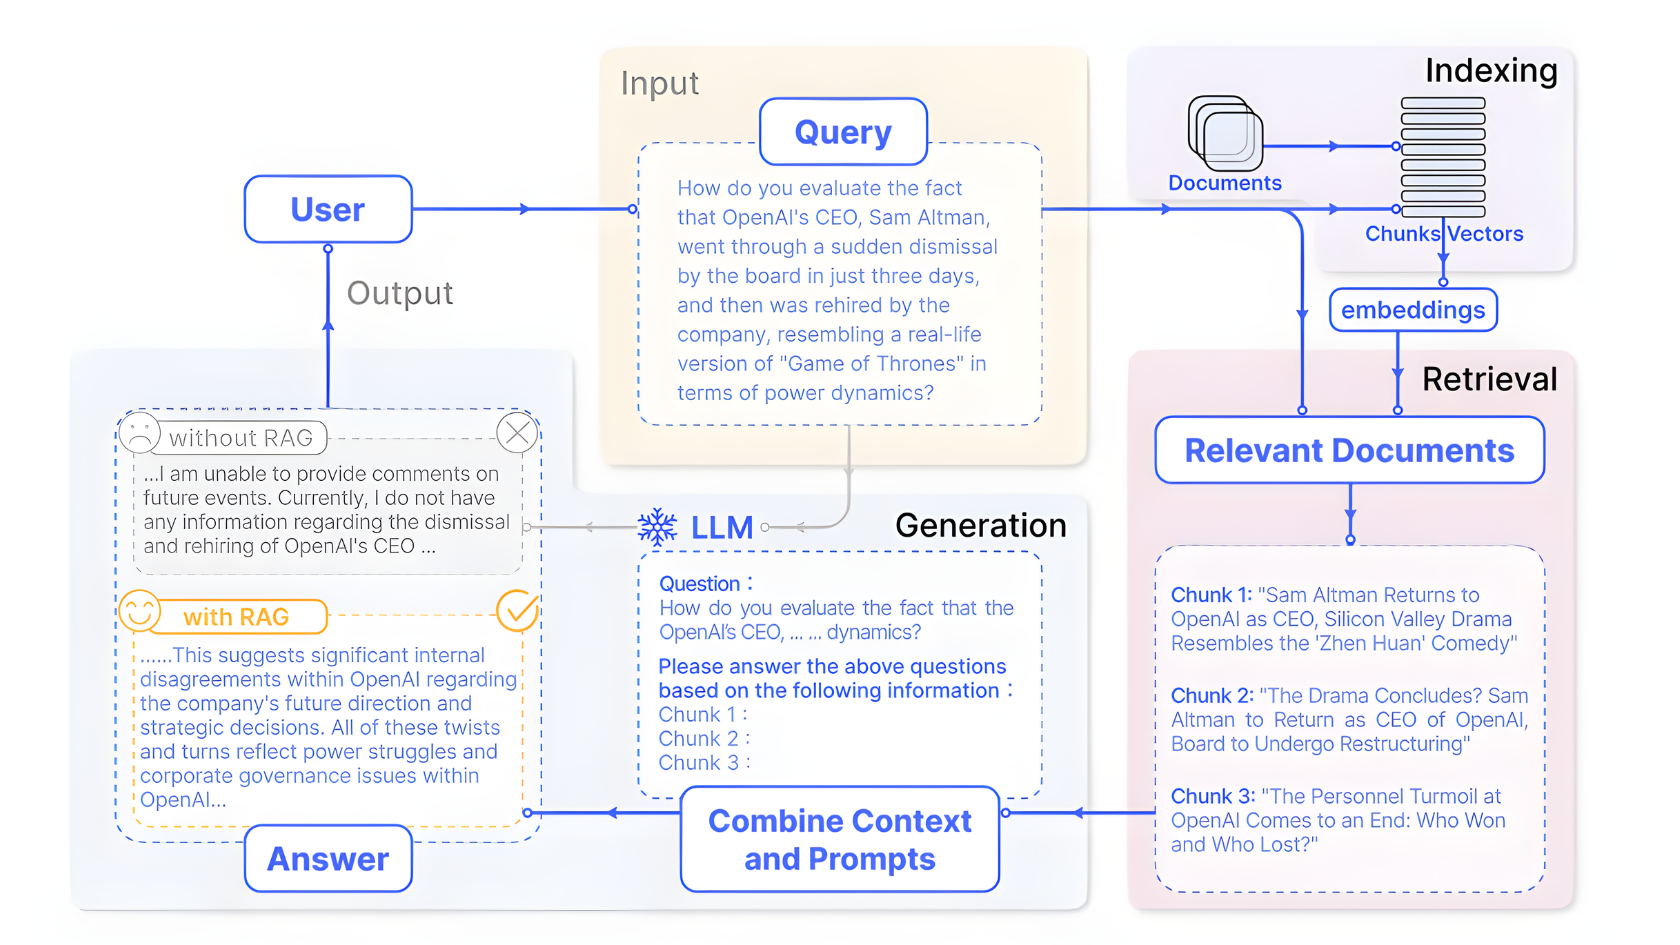
\includegraphics[width=1\textwidth]{Gambar/RAG.png}}
		\caption{Proses Retrieval-Augmented Generation untuk Question Answering \cite{edge2025localglobalgraphrag}}
		\label{fig:rag-process}
\end{figure}

Dengan RAG, LLM bisa secara dinamis memanfaatkan pengetahuan eksternal membuat respons yang dihasilkan menjadi lebih akurat, informatif, dan mutakhir. Proses retrieval mengurangi risiko model "ngarang" jawaban karena jawaban merujuk pada sumber dokumen. Ini membuat RAG sangat unggul dalam domain yang pengetahuannya berkembang cepat, seperti berita, publikasi sains, ataupun regulasi yang berubah secara periodik. Pengguna juga bisa menelusuri dari mana sumber jawaban AI berasal, meningkatkan transparansi dan kepercayaan.
		
Sebagai ilustrasi praktis, misal pengguna ingin mengetahui perkembangan suatu topik berita yang sedang viral beberapa hari terakhir. Model LLM berbasis pre-trained umumnya kurang mampu memberikan informasi terbaru, sehingga respons yang dihasilkan sering kurang relevan dengan konteks aktual. Namun, dengan penerapan skema RAG seperti pada \ref{fig:rag-process}, sistem akan secara otomatis mengambil dan mengintegrasikan dokumen berita terkini sebagai referensi utama, sehingga jawaban yang dihasilkan lebih faktual dan sesuai kebutuhan pengguna.
		
Seiring dengan meningkatnya kebutuhan akan informasi yang akurat dan terkini, RAG telah diintegrasikan dan diadopsi di berbagai bidang aplikasi dalam ekosistem teknologi modern:
\begin{itemize}
	\item \textbf{Open-Domain Question Answering:} RAG terbukti meningkatkan performa QA tanya jawab terbuka karena mampu mengambil referensi dari Wikipedia atau dataset yang relevan, dan secara konsisten melampaui model ekstraktif berbasis machine reading comprehension pada berbagai benchmark seperti pada Natural Questions dan TriviaQA.
	\item \textbf{Aplikasi Legal dan Medis:} Di domain hukum serta kesehatan, RAG digunakan untuk penelusuran dokumen kasus hukum terbaru atau artikel ilmiah medis guna memberi landasan keputusan berbasis data mutakhir dan referensi valid.
	\item \textbf{Chatbot dan Virtual Assistant:} Integrasi RAG pada sistem percakapan seperti ChatGPT memungkinkan respons lebih akurat karena mampu mengambil data keuangan, dokumentasi teknis, ataupun berita terkini secara real-time.
\end{itemize}

\subsection{Graph-Based RAG}

\textit{Graph-RAG} merupakan sebuah evolusi dari arsitektur RAG yang dirancang untuk meningkatkan mekanisme pengambilan informasi dengan memanfaatkan sumber pengetahuan terstruktur, seperti \textit{Knowledge Graph} (KG) atau basis data relasional \cite{peng2024graphretrievalaugmentedgenerationsurvey}. Berbeda dengan RAG konvensional yang umumnya mengambil potongan teks tidak terstruktur, Graph-RAG secara spesifik mengekstraksi elemen-elemen graf yang relevan termasuk entitas, relasi, atau bahkan seluruh subgraf dengan tujuan memperkaya konteks pada \textit{Large Langguage Models} \cite{guo2023gpt4graphlargelanguagemodels}.

\begin{figure}[!t]
    \centering
    % Pastikan path gambar ini sesuai dengan struktur folder di Overleaf Anda
    
\includegraphics[width=1\textwidth]{Gambar/framework graphrag.png}
    \caption{Kerangka kerja GraphRAG untuk tugas menjawab pertanyaan \cite{peng2024graphretrievalaugmentedgenerationsurvey}}
    \label{fig:graphrag-framework}
\end{figure}

Kerangka kerja \textit{Graph-Based RAG} secara garis besar terbagi menjadi tiga tahapan utama yang saling terintegrasi dalam satu alur kerja, sebagaimana diilustrasikan pada \ref{fig:graphrag-framework}:

\begin{itemize}
    \item \textbf{Tahap 1: Indeksasi Berbasis Graf (G-Indexing).}
    Tahap ini berfokus pada pembangunan atau pemilihan basis data graf terstruktur sebagai sumber pengetahuan utama. Proses indeksasi ini bertujuan untuk mengorganisasi entitas (\textit{nodes}) dan relasi (\textit{edges}) sedemikian rupa agar proses penelusuran informasi menjadi lebih efisien. Data graf dapat bersumber dari Graf Pengetahuan terbuka (seperti Wikidata \cite{wikidata}) atau dibangun secara khusus dari \textit{dataset} pribadi sesuai domain yang dituju. \textit{G-Indexing} merupakan fondasi yang krusial karena menentukan tingkat kedetailan dan kualitas data yang dapat diakses pada tahap pengambilan berikutnya, sehingga berperan vital dalam efisiensi sistem secara keseluruhan.
    
    \item \textbf{Tahap 2: Pengambilan Berbasis Graf (G-Retrieval).}
    Berbeda dengan RAG konvensional yang umumnya mengambil penggalan teks yang terpisah, \textit{Graph-Based RAG} dirancang untuk mengekstrak elemen graf yang paling relevan secara kontekstual---baik berupa simpul, triplet relasional (\textit{subject-predicate-object}), lintasan (\textit{paths}), maupun subgraf utuh sesuai dengan kueri pengguna. Metode pengambilan yang digunakan beragam, mulai dari algoritma penelusuran graf tradisional, pencarian kesamaan semantik, hingga model berbasis Jaringan Saraf Graf (GNN). Pemilihan strategi ini sangat bergantung pada karakteristik data graf dan keseimbangan yang diinginkan antara presisi hasil dan efisiensi komputasi.
    
    \item \textbf{Tahap 3: Pembangkitan Respons Berbasis Graf (G-Generation).}
    Pada tahap akhir ini, data graf yang telah diambil diintegrasikan ke dalam proses penyusunan jawaban. Integrasi dapat dilakukan dengan mengubah struktur graf menjadi format narasi tekstual atau dengan memanfaatkan representasi data terstruktur secara langsung melalui model \textit{transformer} yang peka terhadap struktur graf (\textit{graph-aware transformers}) atau model hibrida GNN-LLM. Generator menerima masukan berupa kueri awal, konteks graf yang relevan, serta \textit{prompt} instruksi untuk menghasilkan respons yang koheren, informatif, dan dapat dipertanggungjawabkan validitasnya.
\end{itemize}

Untuk memberikan landasan teoretis bagi tahapan-tahapan praktis yang telah dijelaskan di atas, berikut adalah formulasi matematis yang mendasari kerangka kerja Graph-RAG.

Secara formal, tujuan utama dari proses Graph-RAG adalah mengidentifikasi jawaban optimal $a^*$ untuk suatu kueri $q$, dengan syarat diberikan Graf Pengetahuan target $\mathcal{G}$. Hal ini dinotasikan dalam Persamaan \ref{eq:graphrag_goal}:

\begin{equation}
	a^* = \operatorname*{arg\,max}_{a \in A} p(a|q, \mathcal{G}),
	\label{eq:graphrag_goal}
\end{equation}
di mana $A$ merepresentasikan himpunan seluruh kemungkinan respons yang dapat dihasilkan. Untuk mencapai tujuan tersebut, distribusi probabilitas target $p(a \mid q, \mathcal{G})$ dimodelkan melalui kolaborasi dua komponen utama: model \textit{graph retriever} $p_\theta(G \mid q, \mathcal{G})$ dan model \textit{answer generator} $p_\phi(a \mid q, G)$, di mana $\theta$ dan $\phi$ adalah parameter yang dapat dilatih.

Menggunakan hukum probabilitas total, distribusi $p(a \mid q, \mathcal{G})$ dapat didekomposisi. Namun, mengingat kompleksitas komputasi untuk menelusuri seluruh subgraf yang mungkin, dilakukan pendekatan aproksimasi dengan hanya memilih subgraf paling relevan $G^*$, sebagaimana ditunjukkan pada Persamaan \ref{eq:graphrag_decomposition_approx}:

\begin{equation}
\begin{split}
	p(a \mid q, \mathcal{G}) &= \sum_{G \subseteq \mathcal{G}} p_\phi(a \mid q, G)\, p_\theta(G \mid q, \mathcal{G}) \\
    &\approx p_\phi(a \mid q, G^*)\, p_\theta(G^* \mid q, \mathcal{G}),
\end{split}
\label{eq:graphrag_decomposition_approx}
\end{equation}
dengan $G^*$ menyatakan subgraf yang dianggap paling relevan terhadap kueri $q$ oleh \textit{retriever}. Pendekatan aproksimasi pada baris kedua persamaan di atas memungkinkan model untuk fokus secara efisien pada informasi yang paling instruktif dari seluruh Graf Pengetahuan, sehingga meningkatkan relevansi respons yang dihasilkan tanpa beban komputasi yang berlebihan.

Fondasi matematis dan arsitektural ini memberikan Graph-RAG keunggulan signifikan dibandingkan metode konvensional, meliputi kemampuan penalaran (\textit{reasoning}) yang lebih presisi, peningkatan akurasi faktual, serta interpretasi dan transparansi yang lebih baik. Hal ini dimungkinkan karena respons yang dihasilkan dapat dilacak kembali (\textit{traceable}) ke entitas dan relasi spesifik dalam graf. Karakteristik ini menjadikan Graph-RAG sangat ideal untuk aplikasi yang menuntut konsistensi logika tinggi dan pemahaman mendalam terhadap hubungan antar-entitas.